\begin{center}
\Huge
Partikulære løsninger og integralkurver
\end{center}

\section*{Partikulære løsninger og integralkurver}
\stepcounter{section}

Vi så sidst, at differentialligninger kan have uendeligt mange løsninger nøjagtigt som integraler kan have det. Vi skal i dag arbejde med, hvordan man bestemmer differentialligningsløsninger, der går gennem bestemte punkter. 

\begin{exa}
	Vi betragter differentialligningen 
	\begin{align*}
		y' = xy,
	\end{align*}
	som vi fra sidst husker har den generelle løsning 
	\begin{align*}
		y(x) = ce^{-\frac{1}{2}x^2}.
	\end{align*}
	Vi ønsker at bestemme den differentialligningsløsning, der går gennem punktet $(0,4)$.
	Dette indsættes derfor i løsningen, og vi får
	\begin{align*}
		4=y(0) = ce^{-\frac{1}{2}0^2} = ce^0= c, 
	\end{align*}
	så vi ved, at $c=4$. Vi har derfor den partikulære løsning 
	\begin{align*}
		y(x) = 4e^{-\frac{1}{2}x^2}.
	\end{align*}
	Grafen for en partikulær løsning kaldes for en \textit{integralkurve}, og $y(x)$ er altså
	bestemt, så integralkurven går gennem punktet $(0,4)$.
	Vi kan tegne forskellige løsninger til differentialligningen. Dette kan ses på Figur 
	\ref{fig:diffløsninger}.
	\begin{figure}[H]
		\centering
		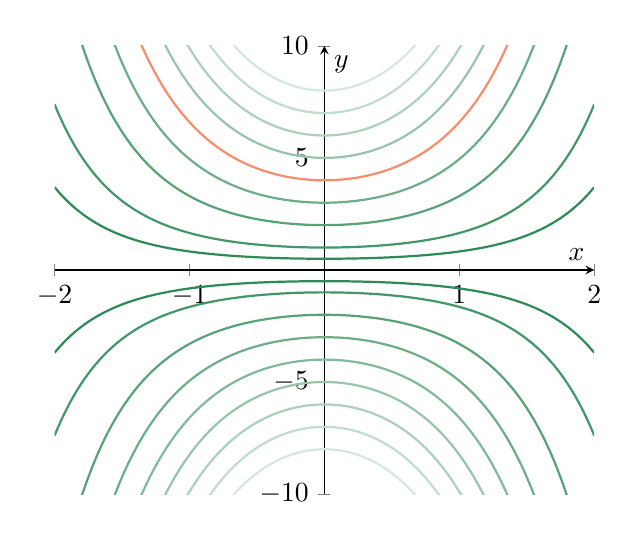
\begin{tikzpicture}
		\begin{axis}[
			axis lines = center, 
			xmin = -2, xmax = 2,
			ymin = -10, ymax = 10,
			xlabel = $x$,
			ylabel = $y$,
		]
			\addplot[color = SeaGreen!20, thick, domain = -2:2, samples = 200] {-8*2.71828^(0.5*x^2)};
			\addplot[color = SeaGreen!30, thick, domain = -2:2, samples = 200] {-7*2.71828^(0.5*x^2)};
			\addplot[color = SeaGreen!40, thick, domain = -2:2, samples = 200] {-6*2.71828^(0.5*x^2)};
			\addplot[color = SeaGreen!50, thick, domain = -2:2, samples = 200] {-5*2.71828^(0.5*x^2)};
			\addplot[color = SeaGreen!60, thick, domain = -2:2, samples = 200] {-4*2.71828^(0.5*x^2)};
			\addplot[color = SeaGreen!70, thick, domain = -2:2, samples = 200] {-3*2.71828^(0.5*x^2)};
			\addplot[color = SeaGreen!80, thick, domain = -2:2, samples = 200] {-2*2.71828^(0.5*x^2)};
			\addplot[color = SeaGreen!90, thick, domain = -2:2, samples = 200] {-1*2.71828^(0.5*x^2)};
			\addplot[color = SeaGreen!100, thick, domain = -2:2, samples = 200] {-0.5*2.71828^(0.5*x^2)};
			\addplot[color = SeaGreen!100, thick, domain = -2:2, samples = 200] {0.5*2.71828^(0.5*x^2)};
			\addplot[color = SeaGreen!90, thick, domain = -2:2, samples = 200] {1*2.71828^(0.5*x^2)};
			\addplot[color = SeaGreen!80, thick, domain = -2:2, samples = 200] {2*2.71828^(0.5*x^2)};
			\addplot[color = SeaGreen!70, thick, domain = -2:2, samples = 200] {3*2.71828^(0.5*x^2)};
			\addplot[color = Melon, thick, domain = -2:2, samples = 200] {4*2.71828^(0.5*x^2)};
			\addplot[color = SeaGreen!50, thick, domain = -2:2, samples = 200] {5*2.71828^(0.5*x^2)};
			\addplot[color = SeaGreen!40, thick, domain = -2:2, samples = 200] {6*2.71828^(0.5*x^2)};
			\addplot[color = SeaGreen!30, thick, domain = -2:2, samples = 200] {7*2.71828^(0.5*x^2)};
			\addplot[color = SeaGreen!20, thick, domain = -2:2, samples = 200] {8*2.71828^(0.5*x^2)};
		\end{axis}
		\end{tikzpicture}
		\caption{Integralkurver for differentialligningen $y' = xy$.}
		\label{fig:diffløsninger}		
	\end{figure}
\end{exa}

\newpage
\begin{exa}
	Vi betragter den simple differentialligning
	\begin{align}\label{eq:1}
		y' = 6x.
	\end{align}
	Vi skal bestemme en løsning til ligningen, så integralkurven for løsningen $f$ går gennem $(2,15)$. 
	Vi bestemmer først den generelle løsning ved at integrere
	\begin{align*}
		\int 6x d x = 3x^2 + k.
	\end{align*}
	Vi indsætter nu punktet.
	\begin{align*}
		15=f(2) = 3(2)^2+k = 12+k,
	\end{align*}
	så $k=3$. 
	Vi har altså bestemt, at den partikulære løsning til \eqref{eq:1} med en integralkurve, 
	der går gennem $(2,15)$ er givet ved 
	\begin{align*}
		f(x) = 3x^2+3.
	\end{align*}
\end{exa}



\subsection*{Opgave 1}
I de følgende to delopgaver skal du bestemme løsninger til differentialligninger ved at integrere.
\begin{enumerate}[label=\roman*)]
	\item Bestem en partikulær løsning til følgende differentialligning, hvis integralkurve
	går gennem punktet $(2,6)$. 
	\begin{align*}
		y' = 5
	\end{align*}
	\item Bestem en partikulær løsning til følgende differentialligning, hvis integralkurve 
	går gennem punktet $(e^{3},16)$.
	\begin{align*}
		y' = \frac{5}{x} 
	\end{align*}
\end{enumerate}

\subsection*{Opgave 2}
	Det oplyses, at 
	\begin{align*}
		y(x) = ce^x-x-1
	\end{align*}
	er den generelle løsning til differentialligningen
	\begin{align}\label{eq:2}
		\frac{d y}{d x} = y+x.
	\end{align}
\begin{enumerate}[label=\roman*)]
\item Vis, at $y(x) = ce^x -x-1$ er en løsning til \eqref{eq:2}.
\item Bestem en løsning til \eqref{eq:2}, der går gennem punktet $(2,3)$.
\end{enumerate}


\subsection*{Opgave 3}
	Det oplyses, at 
	\begin{align*}
		y(x) = cx
	\end{align*}
	er den generelle løsning til differentialligningen
	\begin{align}\label{eq:3}
		y' = \frac{y}{x}
	\end{align}
\begin{enumerate}[label=\roman*)]
\item Vis, at $y(x) = cx$ er en løsning til \eqref{eq:3}.
\item Bestem en løsning til \eqref{eq:3}, der går gennem punktet $(-4,5)$.
\end{enumerate}


\subsection*{Opgave 4}
	Det oplyses, at 
	\begin{align*}
		y(x) = \pm\sqrt{c+x^2}
	\end{align*}
	er den generelle løsning til differentialligningen
	\begin{align}\label{eq:4}
		\frac{d y}{d x} = \frac{x}{y}.
	\end{align}
\begin{enumerate}[label=\roman*)]
\item Vis, at $y(x) = \pm\sqrt{c+x^2}$ er en løsning til \eqref{eq:4}.
\item Bestem en løsning til \eqref{eq:4}, der går gennem punktet $(-4,6)$. (Vælg den positive løsning).
\end{enumerate}


\subsection*{Opgave 5}
	Det oplyses, at 
	\begin{align*}
		y(x) = -\ln(c-e^x)
	\end{align*}
	er den generelle løsning til differentialligningen
	\begin{align}\label{eq:5}
		y'(x) = e^{y+x}.
	\end{align}
\begin{enumerate}[label=\roman*)]
\item Vis, at $y(x) = -\ln(c-e^x)$ er en løsning til \eqref{eq:5}.
\item Bestem en løsning til \eqref{eq:5}, der går gennem punktet $(2,-2)$. 
\end{enumerate}

\subsection*{Opgave 6}

	Det oplyses, at 
	\begin{align*}
		y(x) = c_1e^x+c_2e^{-x}
	\end{align*}
	er den generelle løsning til differentialligningen
	\begin{align}\label{eq:6}
		y'' = y.
	\end{align}
\begin{enumerate}[label=\roman*)]
\item Vis, at $y(x) = c_1e^x+c_2e^{-x}$ er en løsning til \eqref{eq:6}.
\item Bestem en løsning til \eqref{eq:6}, der går gennem punkterne $(0,4)$ og 
$\left(\ln(3), 4\right)$.
\end{enumerate}

\subsection*{Opgave 7}
	Det oplyses, at 
	\begin{align*}
		y(x) = c_1e^{2x}+c_2e^{-x}
	\end{align*}
	er den generelle løsning til differentialligningen
	\begin{align}\label{eq:7}
		y''-y'-2y=0.
	\end{align}
\begin{enumerate}[label=\roman*)]
\item Vis, at $y(x) = c_1e^{2x}+c_2e^{-x}$ er en løsning til \eqref{eq:7}.
\item Bestem en løsning til \eqref{eq:7}, der går gennem punkterne $(0,1)$ og $(\ln(2), 11)$.
\end{enumerate}
